\chapter{Examples of Figures}
\label{cha:important-chapter}
This chapter shows you some examples of figures, such as subfigures,  big, and landscape figures.


\subsection{Just a figure}
As the subsection header states it is just a figure, \ref{fig:Strongbad}. But in the code it does not look like the regular 'figure' input. There is a function that allows you to input a figure, and only have part of the caption shown in the table of content, go ahead and compare the label of \ref{fig:Strongbad} below and the one that popped up in the table of content.

\csmlongfigure{Strongbad}{image-05photo_library_management.png}{2in}{This section of the citation will appear in the List of Figure}{ and this section is added to the citation in the text \cite{cite-xkcd_2017-anotherOne}.}

This function is useful when you have really long figure captions, and you don't need to show all of the description in the table of content.

Now I will add a figure (\ref{fig:CutvsFloatBarrier}) that will be place in the next section somewhere. Lets see what happens when I use Float Barrier.

\begin{figure}[ht]
	\centering
	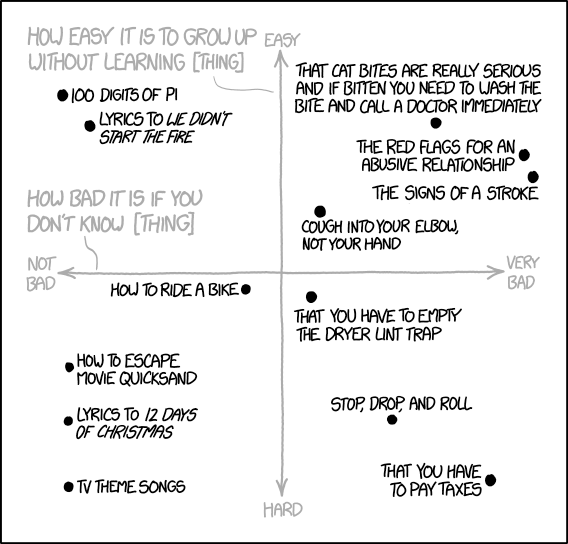
\includegraphics[width = 0.5\textwidth]{image-03.png}
	\caption{Here is a figure that will cut through the next section.}
	\label{fig:CutvsFloatBarrier}
\end{figure}

\FloatBarrier

\subsection{Sub-figures}

Note that both \ref{fig:fsm} and \ref{fig:fsm-2} show the same two figures with sub plots but look different in layout. Also look at where you place the 'label' in the figure, because you can also call one of the subplots, example are \ref{fig:fsm-pirates} and \ref{fig:fsm-pirates2}. The next paragraph is a bunch of non information, only to show where the two figures are going to naturally place themselves.

\begin{figure}
	\centering
	\subfigure[Blue Light with Interference Filter]{
		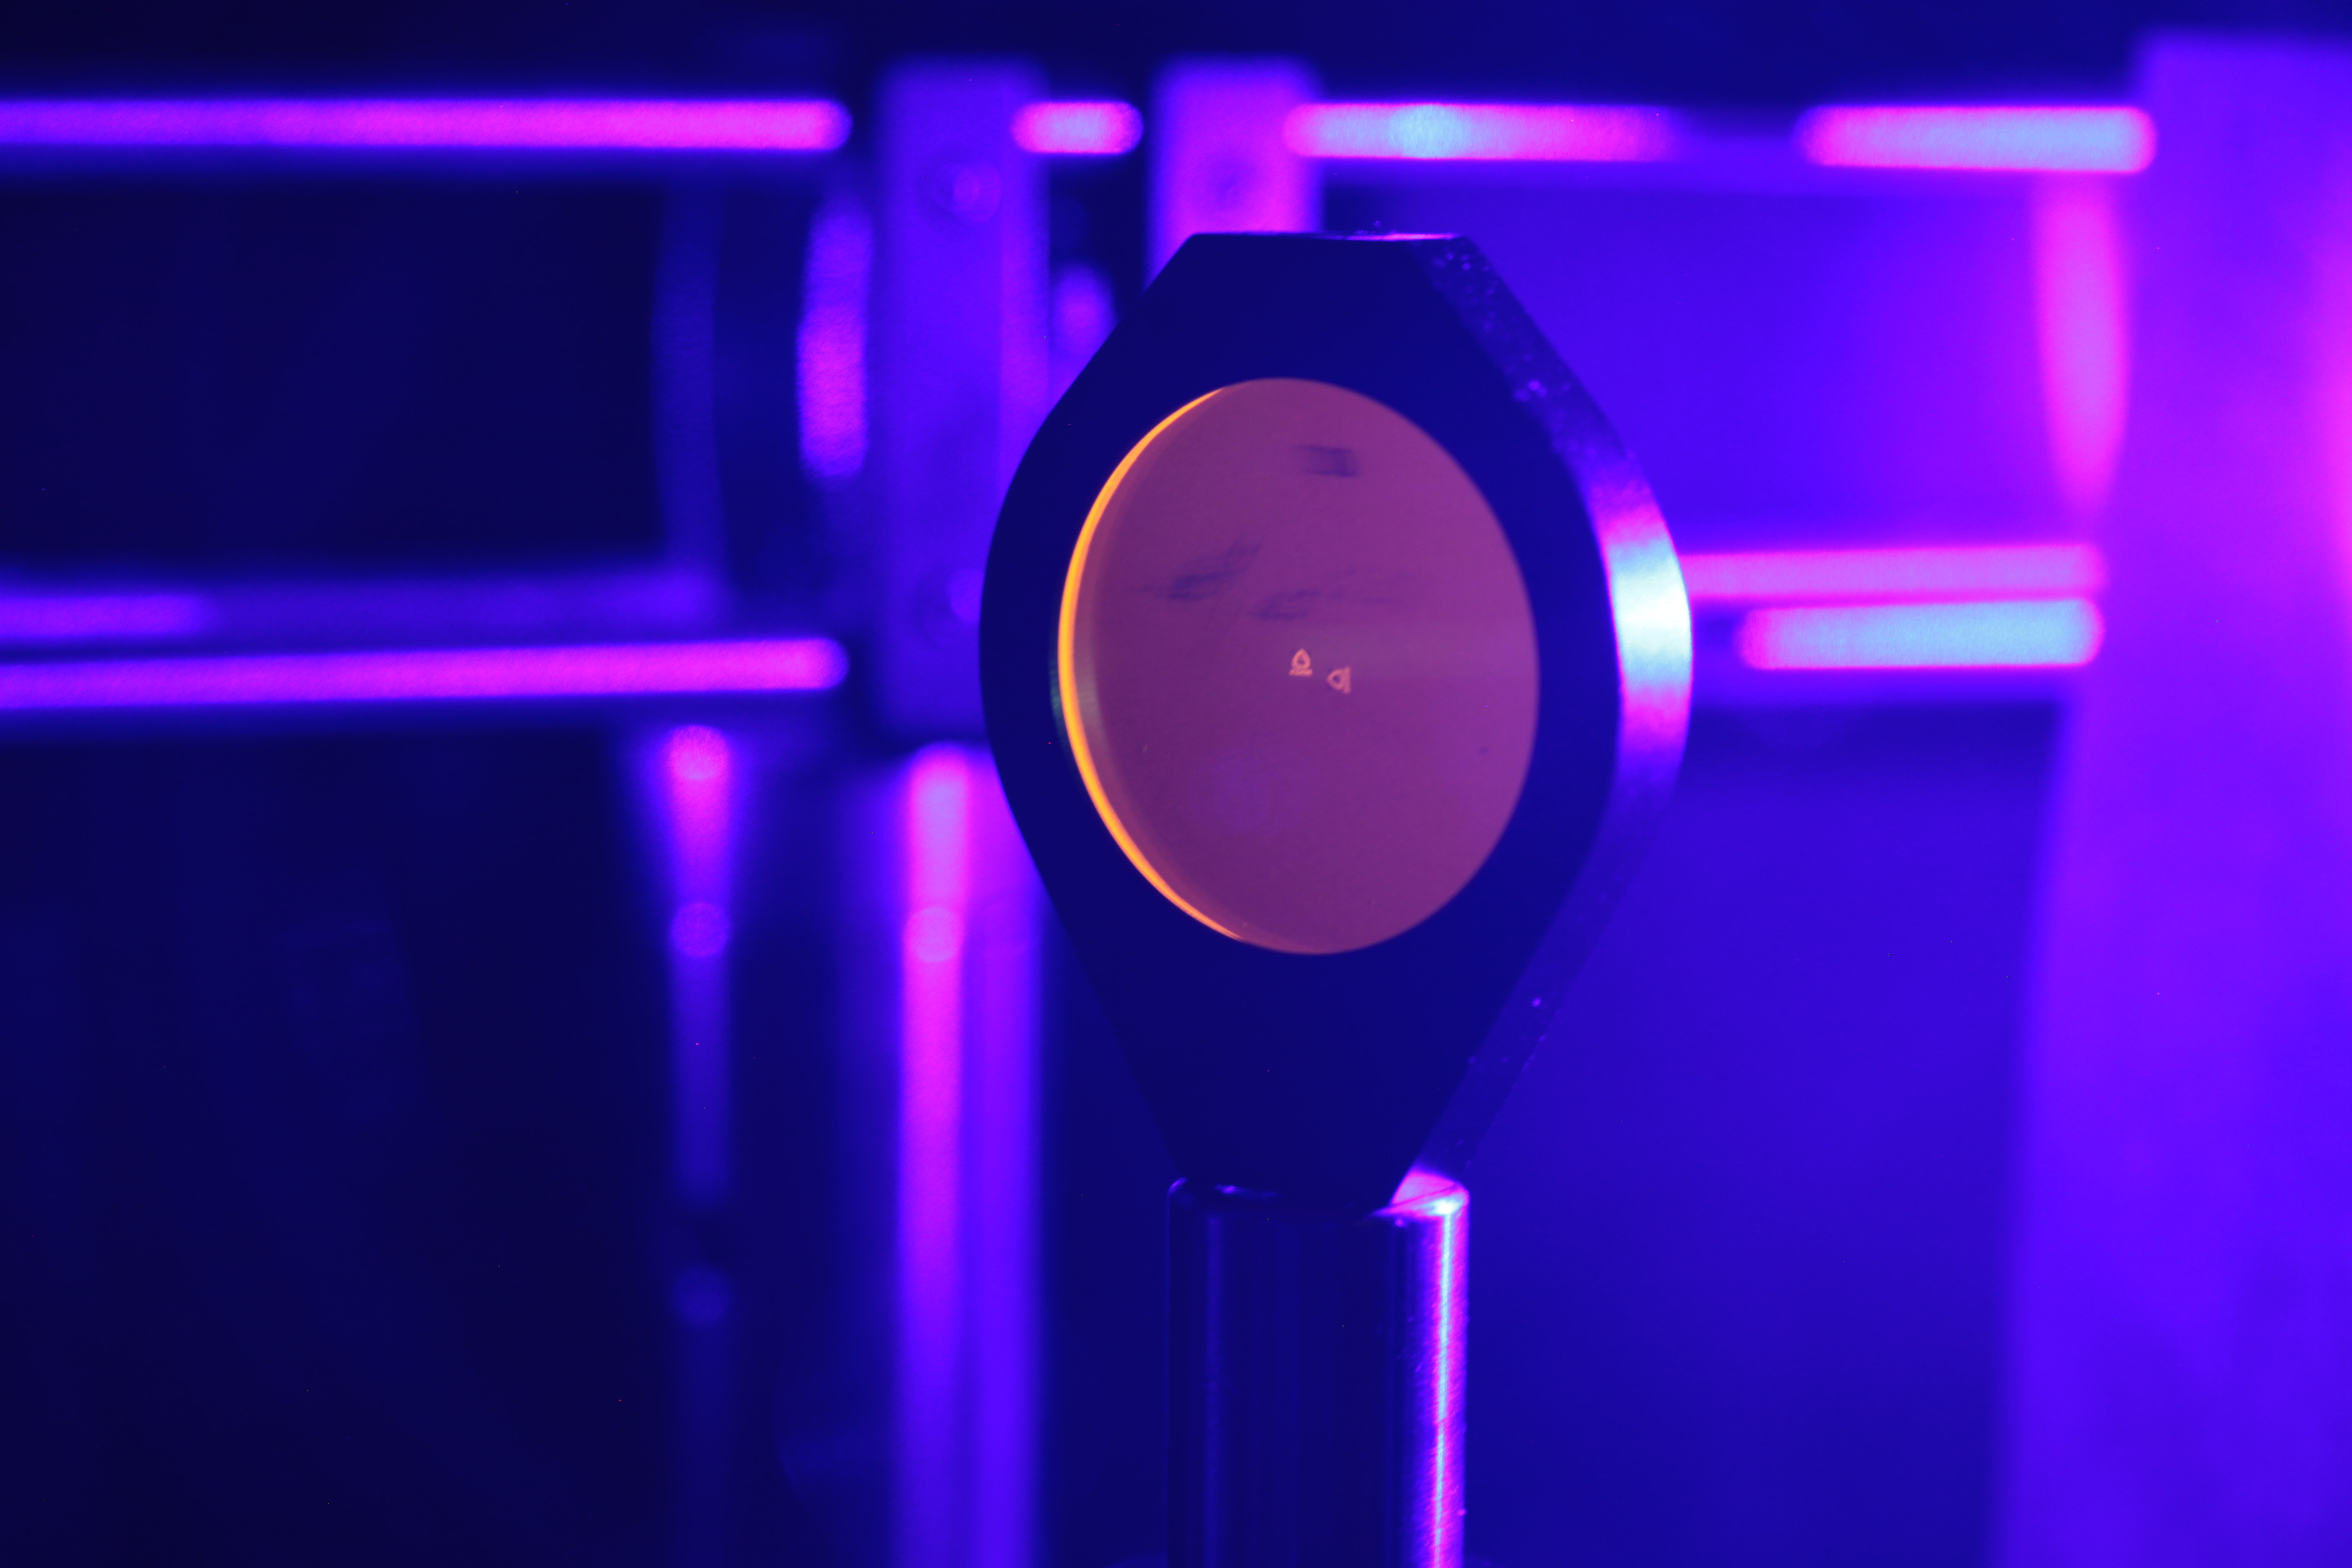
\includegraphics[width=4in]{IMG_2375.JPG}
	} \\
	\subfigure[Cool Sparks]{
		\resizebox{4in}{!}{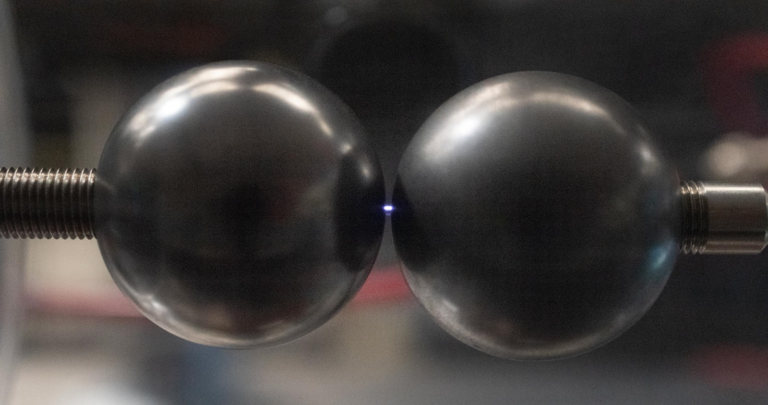
\includegraphics{/try-me/ESD_1600-768x405.png}}
		\label{fig:fsm-pirates}
	}
	\caption{\label{fig:fsm} Here are two images from the Durfee Research Group (a) A reflective object with something engraved in the center \cite{cite-schrama_2019-blue}. (b) A electrostatic discharge event occurring in air taken with a long exposure camera  \cite{cite-schrama_2019}}
\end{figure}

\lipsum[3]

\lipsum[4]

\begin{figure}[ht]
	\centering
	\subfigure[Blue Light with Interference Filter]{
		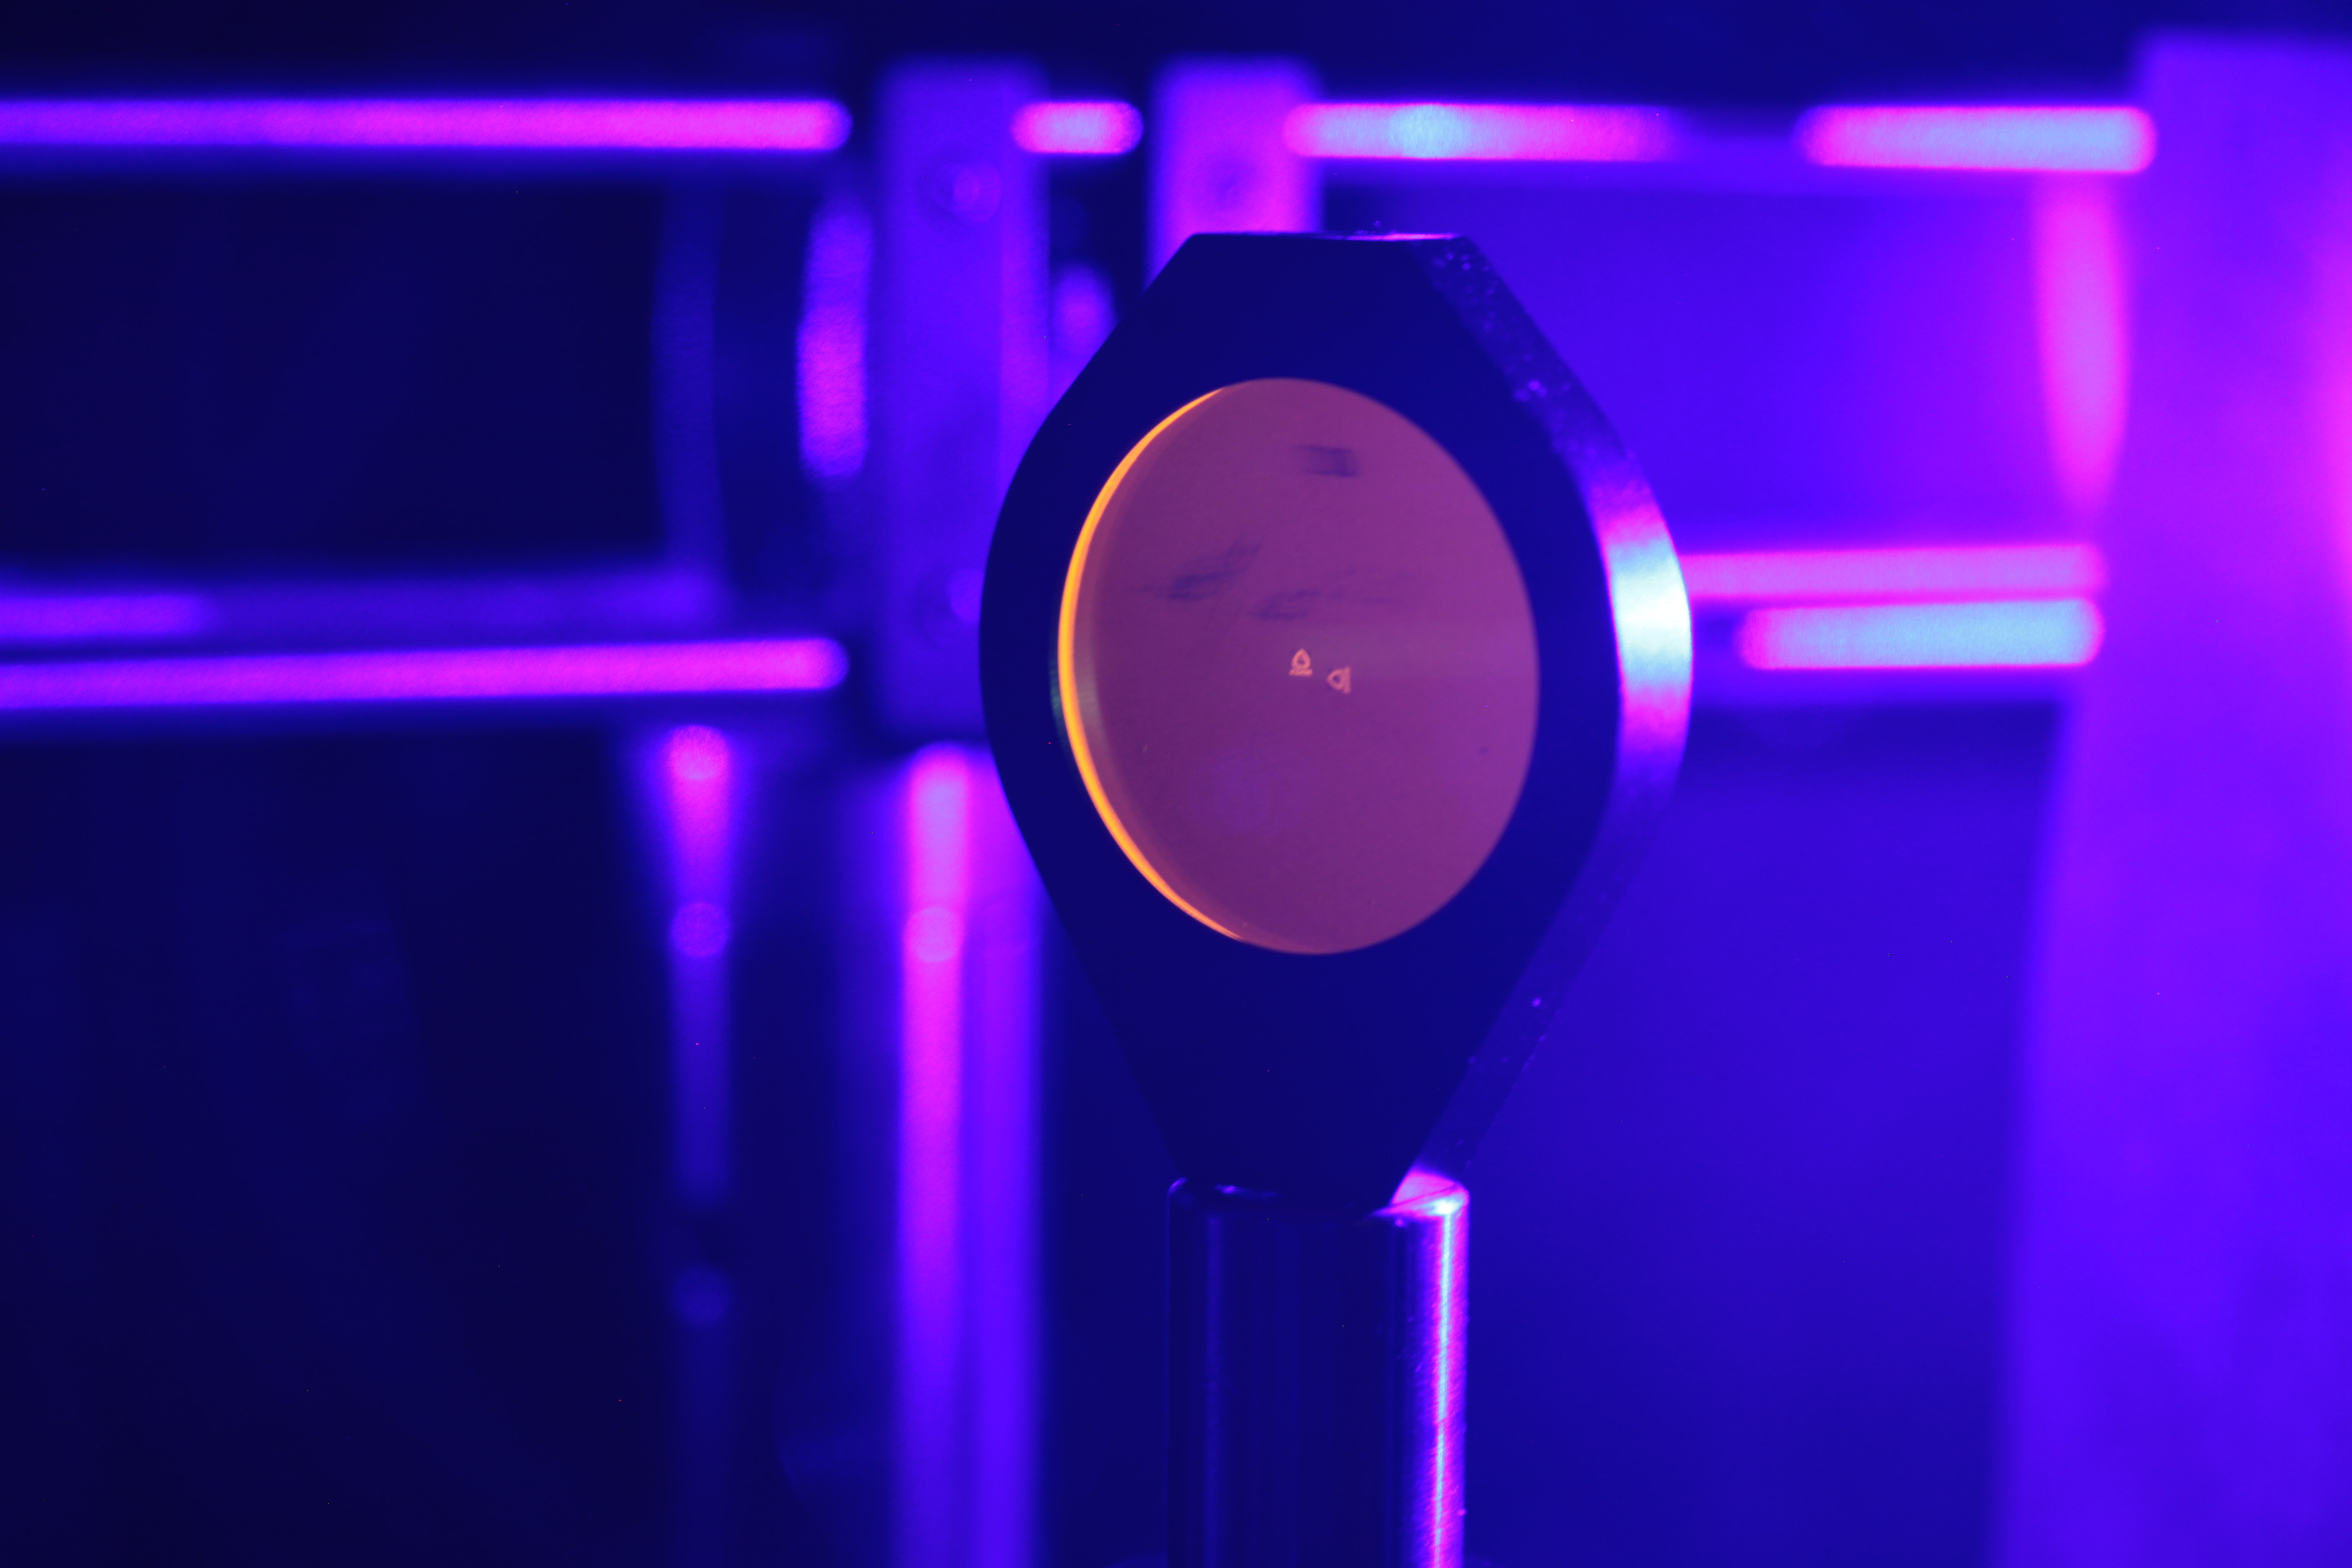
\includegraphics[width=2.5in]{IMG_2375.JPG}
		\label{fig:fsm-pirates2}
	} ~
	\subfigure[Cool Sparks]{
		\resizebox{2.5in}{!}{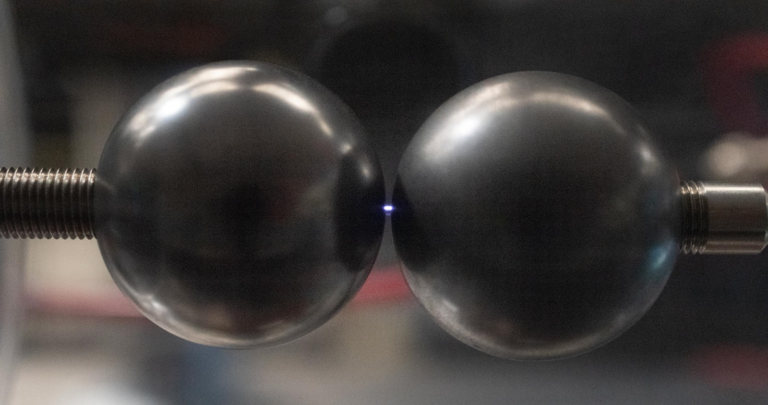
\includegraphics{/try-me/ESD_1600-768x405.png}}

	}

	\caption{\label{fig:fsm-2} Here are two images from the Durfee Research Group (a) A reflective object with something engraved in the center \cite{cite-schrama_2019-blue}. (b) A electrostatic discharge event occurring in air taken with a long exposure camera  \cite{cite-schrama_2019}}
\end{figure}


Notice the the figure with the stacked images places itself on its own page. This figure is greater than 50\% of the page, so if you leave of any placement tags (like [ht]) then most of the time the figure gets moved to it's of page.

\subsection{Landscape Figure}
There is also an example of a really big image following soon that takes up more than 50\% of the page and is in Landscape mode \ref{fig:hallo}. Note that the text wrap does not work around these landscape images, as it did for the above subplot, because Section \ref{sec-Important} should be right after this line. This means you need to think about where you place these landscape figures (or tables).

\begin{landscape}
	\centering
	\begin{figure}[ht]
		\centering
		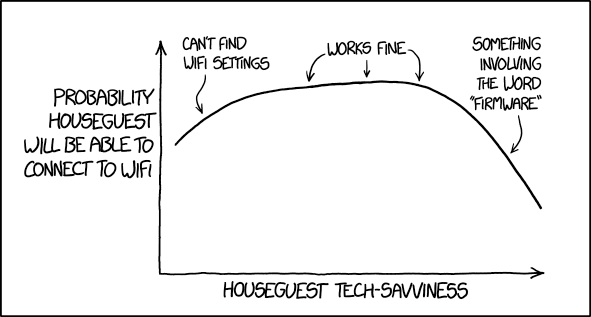
\includegraphics[width=\linewidth]{image-04.png}
		\caption{This is an example of a landscape page filled by a picture.}
		\label{fig:hallo}
	\end{figure}
\end{landscape}

\subsection{Here is an example that does not always work} \label{sec-Important}
We thought that was the end! But here I have placed a figure, \ref{fig:hallo2}, and it should pushes itself to its own page after this page is filled up all the way. If you comment out the paragraph between here and the figure you will see that the figure is placed wrong (and got rid of the [p] on the figure).

\lipsum[1]

\begin{figure}[p]
	\centering
	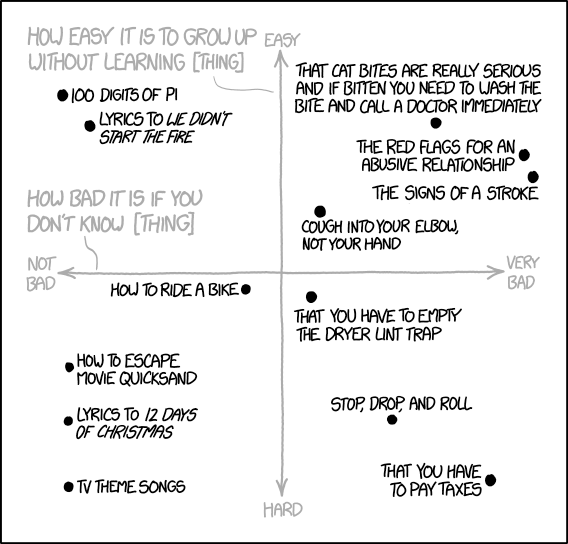
\includegraphics[width = \textwidth]{image-03.png}
	\caption{This figure will show after the current page has ended and only contain this figure on the page. \cite{cite-xkcd_2016}}
	\label{fig:hallo2}
\end{figure}

\lipsum[2]

\lipsum[3]

\lipsum[1]

Here is an example of a caption and a other thins \ref{fig:WayToBig}

\clearpage

\begin{figure}[p]
	\centering
	\caption{Here is a really long caption for the figure that will follow on the next page. So I have to make this caption really long. I can get this system to work but unfortunately the user will have to pay extra attention to the text wrapping because it will not do it one its own !!! This is very important. The figure is actually outside of the figure environment. So Clear the page, then insert the caption and label in the figure environment, and then clear the page again. This way you can add the [p] placement marker which will center the caption vertically on the page. Next add the figure after the second clear page with only include graphics and not in any figure environment. The image is one made by the author of this template document, Claudia Schrama, where a Moku:Lab instrument is used to analyze a circuit using the frequency response analyzer function. }
	\label{fig:WayToBig}
\end{figure}

\clearpage

\vspace*{\fill}
\begin{center}
	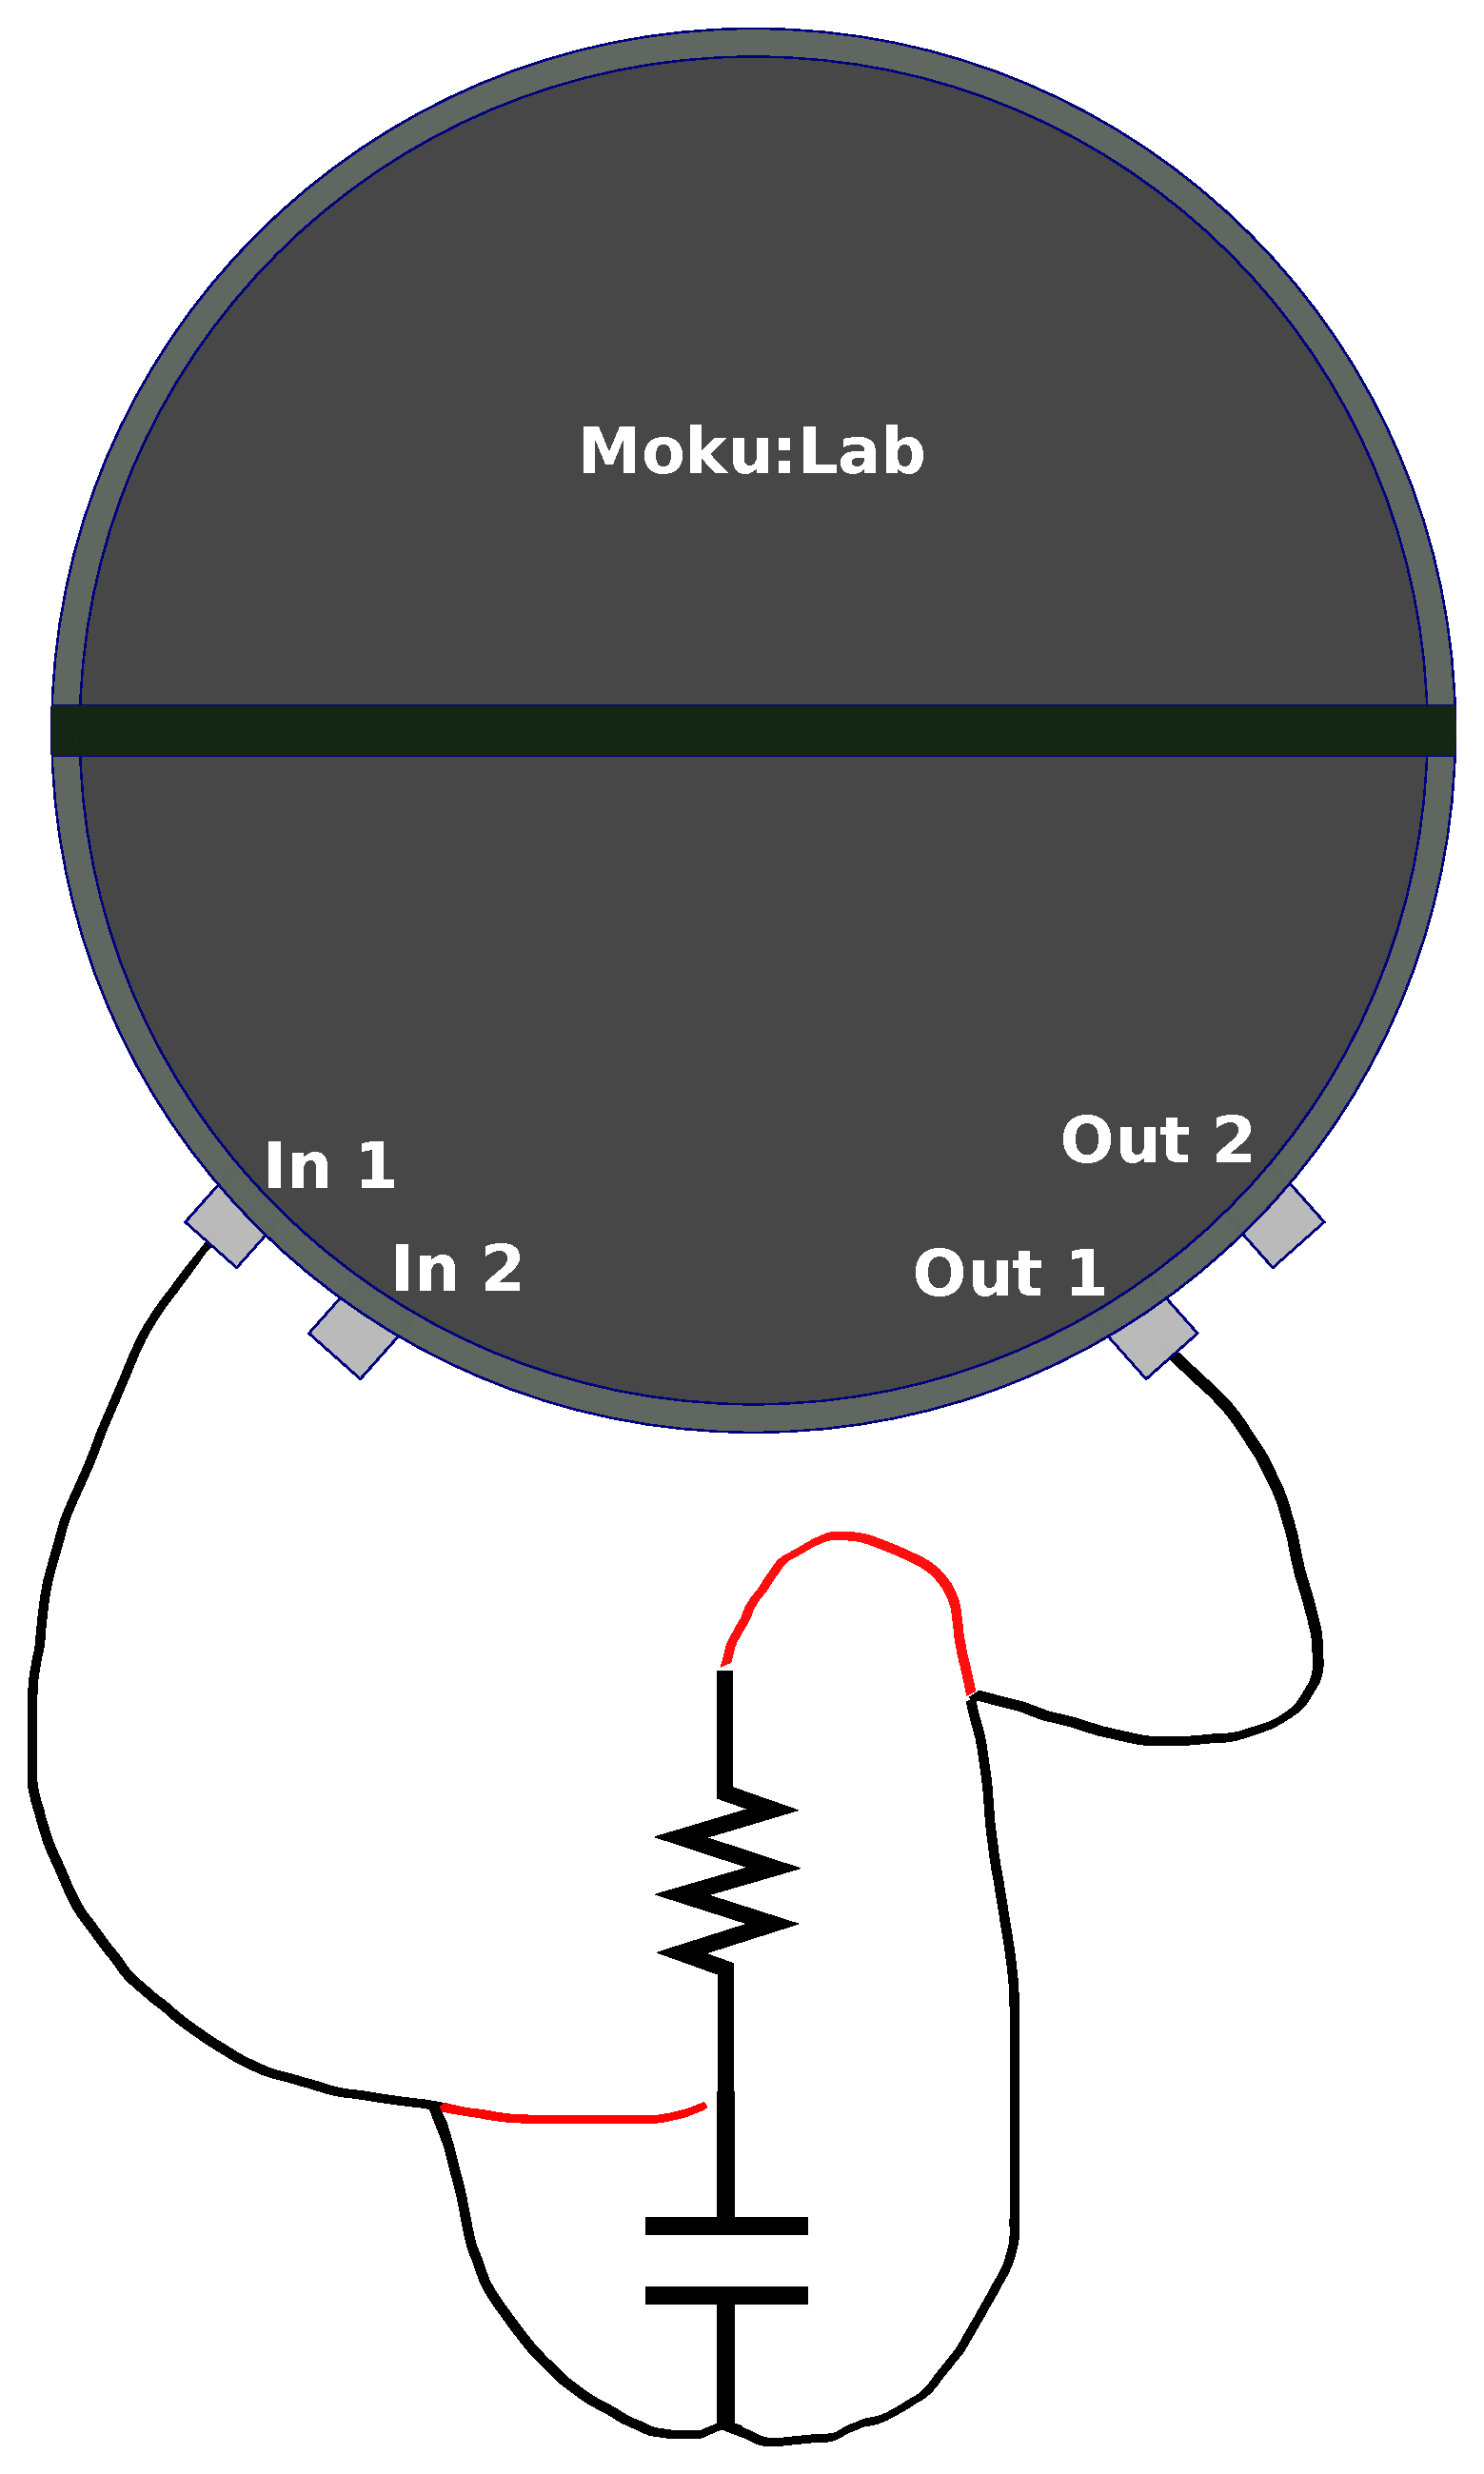
\includegraphics[height =0.9 \textheight]{20120-04-16-YoutubeLiquidInstuments.pdf}
\end{center}
\vspace*{\fill}

\clearpage


% \csmsplitfigure{yep}{Caption This}{!}{image-03.png}
